\section{真实运行结果与诊断}

\begin{frame}{验证基线：当前工作树的规定测试与冒烟均通过}
\centering
\metric{86}{passed}\hfill
\metric{0}{failed}\hfill
\metric{10.09 s}{pytest}\hfill
\metric{PASS}{smoke pipeline}

\vspace{1.2em}
\begin{block}{执行命令}
\small\ttfamily
uv run pytest backend/intel\_agent/tests backend/ctinexus\_kg/tests backend/console/tests -q

uv run python scripts/smoke\_pipeline.py
\end{block}

\begin{columns}[T,onlytextwidth]
\column{0.48\textwidth}
\begin{exampleblock}{测试证明了什么}
schema、算法、fallback、工具约束、存储、UI 组件及 fake KG 交接的已编码不变量没有回归。
\end{exampleblock}
\column{0.48\textwidth}
\begin{alertblock}{没有证明什么}
真实外部源 recall、人工 precision、跨 provider 稳定性、长时 full campaign、恶意内容安全和全局 KG 质量。
\end{alertblock}
\end{columns}
\end{frame}

\begin{frame}{Mongo 历史：规模已形成，但来源高度偏向 arXiv}
\begin{columns}[T,onlytextwidth]
\column{0.62\textwidth}
\begin{tikzpicture}
\begin{axis}[
  xbar,
  width=8.0cm,height=5.2cm,
  xmin=0,xmax=5800,
  symbolic y coords={CISA,OSV,NVD,arXiv},
  ytick=data,
  xlabel={全局去重 items},
  nodes near coords,
  nodes near coords align={horizontal},
  bar width=10pt,
  axis line style={draw=Slate},
  tick label style={font=\scriptsize},
  label style={font=\scriptsize},
  enlarge y limits=0.15
]
\addplot[fill=Blue,draw=Blue] coordinates {(268,CISA) (536,OSV) (936,NVD) (5209,arXiv)};
\end{axis}
\end{tikzpicture}
\column{0.34\textwidth}
\begin{block}{统一快照}
\begin{itemize}
  \item 12 runs
  \item 6,949 distinct items
  \item 2,505 items 跨 run 重现
  \item 3 item-KGs
\end{itemize}
\end{block}
\begin{alertblock}{来源占比}
arXiv 75.0\%；NVD 13.5\%；OSV 7.7\%；CISA 3.9\%。高吞吐 research 通道主导 corpus。
\end{alertblock}
\end{columns}
\smallsource{Mongo \pathcode{intel_agent}，2026-07-15 12:48 UTC；\pathcode{runtime_snapshot.json}}
\end{frame}

\begin{frame}{主题分布：头部充足，部分 Core 几乎没有证据}
\small
\begin{columns}[T,onlytextwidth]
\column{0.58\textwidth}
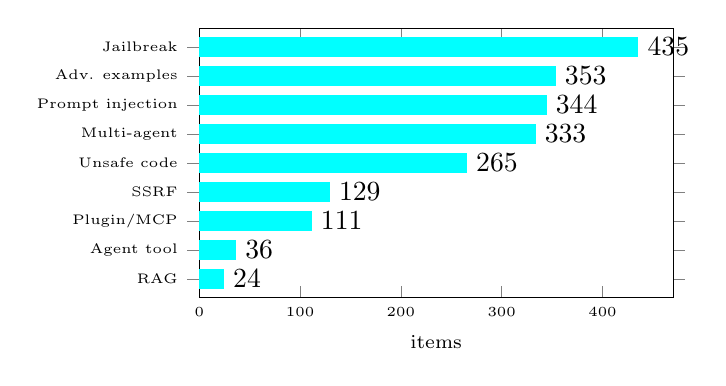
\begin{tikzpicture}
\begin{axis}[
  xbar,width=7.6cm,height=5.0cm,
  xmin=0,xmax=470,
  symbolic y coords={RAG,Agent tool,Plugin/MCP,SSRF,Unsafe code,Multi-agent,Prompt injection,Adv. examples,Jailbreak},
  ytick=data,nodes near coords,bar width=7pt,
  tick label style={font=\tiny},label style={font=\scriptsize},
  xlabel={items},enlarge y limits=0.08
]
\addplot[fill=Cyan,draw=Cyan] coordinates {
  (24,RAG) (36,Agent tool) (111,Plugin/MCP) (129,SSRF) (265,Unsafe code)
  (333,Multi-agent) (344,Prompt injection) (353,Adv. examples) (435,Jailbreak)};
\end{axis}
\end{tikzpicture}
\column{0.38\textwidth}
\begin{alertblock}{弱覆盖主题}
\scriptsize
\begin{tabular}{lr}
excessive agency & 6\\
unbounded consumption & 6\\
insecure output handling & 4\\
model denial of service & 2\\
logging/monitoring & 1\\
misinformation/citation & 1\\
internal recon & 1\\
\end{tabular}
\end{alertblock}
\begin{block}{不能仅看 count}
这些是主题标签 item 数，不等于独立事件数或有效证据；但长尾足以说明固定查询策略存在结构性盲点。
\end{block}
\end{columns}
\end{frame}

\begin{frame}{相关性测量：67.4\% 为 uncertain，LLM 复核仅占 0.35\%}
\small
\begin{columns}[T,onlytextwidth]
\column{0.46\textwidth}
\begin{block}{标签分布（6,949）}
\begin{tabularx}{0.96\linewidth}{X r r}
\toprule
label & count & share \\
\midrule
uncertain & 4,683 & 67.39\% \\
relevant & 2,157 & 31.04\% \\
irrelevant & 109 & 1.57\% \\
\bottomrule
\end{tabularx}
\end{block}
\column{0.46\textwidth}
\begin{block}{决策方法}
\begin{tabularx}{0.96\linewidth}{X r r}
\toprule
method & count & share \\
\midrule
rule & 5,976 & 86.00\% \\
embedding & 949 & 13.66\% \\
LLM & 24 & 0.35\% \\
\bottomrule
\end{tabularx}
\end{block}
\end{columns}

\begin{alertblock}{诊断}
系统不是“缺少分类结果”，而是大量样本落在灰区。下一步不是简单放宽阈值，而是抽样标注、校准 score、核对 escalation 配置和 LLM batch 实际触发率。
\end{alertblock}
\end{frame}

\begin{frame}{最新 full/bootstrap：能正常停止，但覆盖结构明显不足}
\centering
\metric{3}{rounds}\hfill
\metric{12}{source API calls}\hfill
\metric{28}{items}\hfill
\metric{229.7 s}{elapsed}

\vspace{0.9em}
\begin{tikzpicture}[
  n/.style={draw,rounded corners,minimum width=3.0cm,minimum height=1.0cm,align=center,font=\scriptsize,thick},
  a/.style={-{Latex[length=1.7mm]},thick,Navy}
]
\node[n,fill=SoftGreen] (r1) {Round 1\\new relevant/call 6.25\\continue};
\node[n,fill=SoftAmber,right=0.8cm of r1] (r2) {Round 2\\new relevant/call 0.25\\continue};
\node[n,fill=SoftRed,right=0.8cm of r2] (r3) {Round 3\\new relevant/call 0.00\\STOP};
\draw[a] (r1)--(r2);\draw[a] (r2)--(r3);
\end{tikzpicture}

\vspace{0.7em}
\begin{columns}[T,onlytextwidth]
\column{0.47\textwidth}
\begin{block}{事实}
28 条全部来自 NVD；仅使用 1 个 source；15/18 Core legacy 配额仍未满足；最后动作 STOP。
\end{block}
\column{0.49\textwidth}
\begin{alertblock}{schema 反例}
summary 同时给出 \pathcode{core_gap_count=0}、15 个 \pathcode{coverage_gaps_remaining}、\pathcode{stop_reason=null}。前者不能被用作“覆盖完成”。
\end{alertblock}
\end{columns}
\smallsource{run \pathcode{real-intel-agent-bootstrap-20260715T120801Z}}
\end{frame}

\begin{frame}{最新 trace：137 个事件可回放，SDK 成本约 0.475 美元}
\begin{columns}[T,onlytextwidth]
\column{0.57\textwidth}
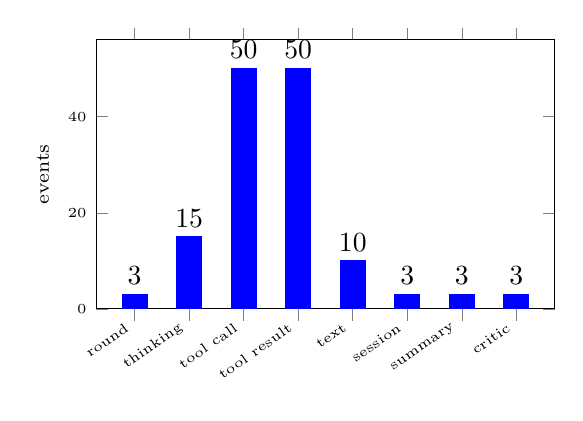
\begin{tikzpicture}
\begin{axis}[
  ybar,width=7.4cm,height=5.0cm,ymin=0,ymax=56,
  symbolic x coords={round,thinking,tool call,tool result,text,session,summary,critic},
  xtick=data,xticklabel style={rotate=35,anchor=east,font=\tiny},
  nodes near coords,bar width=9pt,
  tick label style={font=\tiny},label style={font=\scriptsize},ylabel={events}
]
\addplot[fill=Blue,draw=Blue] coordinates {(round,3) (thinking,15) (tool call,50) (tool result,50) (text,10) (session,3) (summary,3) (critic,3)};
\end{axis}
\end{tikzpicture}
\column{0.39\textwidth}
\begin{block}{Session 汇总}
\begin{itemize}
  \item SDK turns：53
  \item cost：\$0.47506
  \item session errors：0
  \item trace file：同 run ID JSONL
\end{itemize}
\end{block}
\begin{alertblock}{不要相除}
50 个 tool calls 并非 50 个源请求；blackboard 的源 API calls 是 12。
\end{alertblock}
\end{columns}
\end{frame}

\begin{frame}{根因链：最新结果不是单点故障，而是路径与目标不一致}
\centering
\begin{tikzpicture}[
  n/.style={draw,rounded corners,minimum width=2.4cm,minimum height=0.8cm,align=center,font=\scriptsize,thick},
  a/.style={-{Latex[length=1.7mm]},thick,Red},node distance=0.42cm
]
\node[n,fill=SoftRed] (goal) {用户目标：完整\\LLM 安全初始语料};
\node[n,fill=SoftAmber,right=of goal] (mode) {选择 full\\但 full=legacy quota};
\node[n,fill=SoftAmber,right=of mode] (query) {本轮策略集中 NVD\\无 source diversity};
\node[n,fill=SoftAmber,right=of query] (stop) {边际 yield 下降\\critic STOP};
\node[n,fill=SoftRed,right=of stop] (out) {28 items\\15 gap 未满足};
\draw[a] (goal)--(mode);\draw[a] (mode)--(query);\draw[a] (query)--(stop);\draw[a] (stop)--(out);
\end{tikzpicture}

\vspace{1em}
\begin{block}{Why-Why 结论}
停止本身符合 legacy 低收益规则；真正的问题是 full 的 measurement/coverage contract 没有表达“每个主题需要哪些证据通道、多少独立事件、何种新鲜度”，所以 controller 无法把业务目标转成可验证终态。
\end{block}
\end{frame}

\begin{frame}{运行结论：可用性不是“能跑”，而是稳定交付满足合同的 corpus}
\begin{columns}[T,onlytextwidth]
\column{0.48\textwidth}
\begin{exampleblock}{当前可称为成熟的部分}
\begin{itemize}
  \item 软件边界与测试基线
  \item 多源连接、解析、去重与持久化
  \item SDK 白名单、hook、trace、fallback
  \item adaptive 算法组件已编码
\end{itemize}
\end{exampleblock}
\column{0.48\textwidth}
\begin{alertblock}{尚不能宣称成熟的部分}
\begin{itemize}
  \item full/bootstrap 的有效覆盖与可恢复性
  \item relevance/topic measurement validity
  \item 同预算下 adaptive 的增益与统计显著性
  \item 新主题真实 precision
  \item item-KG 到 global KG 的质量闭环
\end{itemize}
\end{alertblock}
\end{columns}

\vspace{0.5em}
\begin{center}
\Large 北极星：\textcolor{Purple}{固定预算下，交付质量验证、结构覆盖、可恢复且可追溯的初始语料库}
\end{center}
\end{frame}
